%  LaTeX support: latex@mdpi.com 
%  In case you need support, please attach all files that are necessary for compiling as well as the log file, and specify the details of your LaTeX setup (which operating system and LaTeX version / tools you are using).

%=================================================================
\documentclass[sensors,article,submit,moreauthors]{Definitions/mdpi} 

% If you would like to post an early version of this manuscript as a preprint, you may use preprint as the journal and change 'submit' to 'accept'. The document class line would be, e.g., \documentclass[preprints,article,accept,moreauthors,pdftex]{mdpi}. This is especially recommended for submission to arXiv, where line numbers should be removed before posting. For preprints.org, the editorial staff will make this change immediately prior to posting.

%--------------------
% Class Options:
%--------------------
%----------
% journal
%----------
% Choose between the following MDPI journals:
% biologics, jmp, eng, jor, nursrep, biophysica, gastroent, jox, adolescents, hygiene, taxonomy, business, nanomanufacturing, geography, compoundsacoustics, actuators, addictions, admsci, aerospace, agriculture, agriengineering, agronomy, ai, algorithms, allergies, analytica, animals, antibiotics, antibodies, antioxidants, applmech, applnano, applsci, arts, asc, asi, atmosphere, atoms, automation, axioms, batteries, bdcc, behavsci , beverages, bioengineering, biology, biomedicines, biomedinformatics, biomimetics, biomolecules, biosensors, bloods, brainsci, breath, buildings, cancers, carbon , catalysts, cells, ceramics, challenges, chemengineering, chemistry, chemosensors, chemproc, children, civileng, cleantechnol, climate, clockssleep, cmd, coatings, colloids, computation, computers, condensedmatter, cosmetics, cryptography, crystals, cyber, dairy, data, dentistry, dermatopathology, designs, diabetology, diagnostics, digital, diseases, diversity, drones, earth, econometrics, ecologies, economies, education, ejbc, ejihpe, electricity, electrochem, electronicmat, electronics, endocrines, energies, engproc, entropy, environments, environsciproc, epidemiologia, epigenomes, est, fermentation, fibers, fire, fishes, fluids, foods, forecasting, forests, fractalfract, fuels, futureinternet, futurephys, galaxies, games, gardens, gases, gastrointestdisord, gels, genealogy, genes, geohazards, geosciences, geriatrics, hazardousmatters, healthcare, hearts, heritage, highthroughput, horticulturae, humanities, hydrogen, hydrology, ijerph, ijfs, ijgi, ijms, ijtpp, immuno, informatics, information, infrastructures, inorganics, insects, instruments, inventions, iot, j, jcdd, jce, jcm, jcp, jcs, jdb, jfb, jfmk, jimaging, jintelligence, jlpea, jmmp, jmse, jne, jnt, jof, joitmc, journalmedia, jpm, jrfm, jsan, land, languages, laws, life, literature, livers, logistics, lubricants, machines, magnetochemistry, make, marinedrugs, materials, materproc, mathematics, mca, medicina, medicines, medsci, membranes, metabolites, metals, microarrays, micromachines, microorganisms, minerals, modelling, molbank, molecules, mps, mti, nanomaterials, ncrna, ijns, neurosci, neuroglia, nitrogen, notspecified, nutrients, obesities, oceans, ohbm, osteology, optics, organics, particles, pathogens, pharmaceuticals, pharmaceutics, pharmacy, philosophies, photonics, physics, plants, plasma, pollutants, polymers, polysaccharides, preprints , proceedings, processes, prosthesis, proteomes, psych, psychiatryint, publications, quantumrep, quaternary, qubs, radiation, reactions, recycling, religions, remotesensing, reprodmed, reports, resources, risks, robotics, safety, sci, scipharm, sensors, separations, sexes, signals, sinusitis, skins, smartcities, sna, societies, socsci, soilsystems, solids, sports, standards, stats, surfaces, surgeries, suschem, sustainability, world, symmetry, systems, technologies, telecom, test, tourismhosp, toxics, toxins, transplantology, tropicalmed, universe, urbansci, uro, vaccines, vehicles, vetsci, vibration, viruses, vision, water, wem, wevj, women

%---------
% article
%---------
% The default type of manuscript is "article", but can be replaced by: 
% abstract, addendum, article, benchmark, book, bookreview, briefreport, casereport, changes, comment, commentary, communication, conceptpaper, conferenceproceedings, correction, conferencereport, expressionofconcern, extendedabstract, meetingreport, creative, datadescriptor, discussion, editorial, essay, erratum, hypothesis, interestingimages, letter, meetingreport, newbookreceived, obituary, opinion, projectreport, reply, retraction, review, perspective, protocol, shortnote, supfile, technicalnote, viewpoint
% supfile = supplementary materials

%----------
% submit
%----------
% The class option "submit" will be changed to "accept" by the Editorial Office when the paper is accepted. This will only make changes to the frontpage (e.g., the logo of the journal will get visible), the headings, and the copyright information. Also, line numbering will be removed. Journal info and pagination for accepted papers will also be assigned by the Editorial Office.

%------------------
% moreauthors
%------------------
% If there is only one author the class option oneauthor should be used. Otherwise use the class option moreauthors.

%---------
% pdftex
%---------
% The option pdftex is for use with pdfLaTeX. If eps figures are used, remove the option pdftex and use LaTeX and dvi2pdf.

%=================================================================
\firstpage{1} 
\makeatletter 
\setcounter{page}{\@firstpage} 
\makeatother
\pubvolume{xx}
\issuenum{1}
\articlenumber{5}
\pubyear{2020}
\copyrightyear{2020}
%\externaleditor{Academic Editor: name}
\history{Received: date; Accepted: date; Published: date}
%\updates{yes} % If there is an update available, un-comment this line

%% MDPI internal command: uncomment if new journal that already uses continuous page numbers 
%\continuouspages{yes}

%------------------------------------------------------------------
% The following line should be uncommented if the LaTeX file is uploaded to arXiv.org
%\pdfoutput=1

%=================================================================
% Add packages and commands here. The following packages are loaded in our class file: fontenc, inputenc, calc, indentfirst, fancyhdr, graphicx,epstopdf, lastpage, ifthen, lineno, float, amsmath, setspace, enumitem, mathpazo, booktabs, titlesec, etoolbox, tabto, xcolor, soul, multirow, microtype, tikz, totcount, amsthm, hyphenat, natbib, hyperref, footmisc, url, geometry, newfloat, caption

%=================================================================
% Graphics path for generated publication figures
\graphicspath{{../../../../../results/for_submission/}{../../../../../results/Sensors_figures/}{../../../../../results/publication_figures/}{../../../../../results/plots/}}
% Prefer PDF/PNG (XeLaTeX compatible)
\DeclareGraphicsExtensions{.pdf,.png}
% Chinese support for XeLaTeX
\usepackage{fontspec}
\usepackage{xeCJK}
\setCJKmainfont{Microsoft YaHei}
\setCJKsansfont{Microsoft YaHei}
% Western text font to support Greek symbols
% Use a Palatino-family font to align with MDPI's Palatino style
\setmainfont{Palatino Linotype}
%% Please use the following mathematics environments: Theorem, Lemma, Corollary, Proposition, Characterization, Property, Problem, Example, ExamplesandDefinitions, Hypothesis, Remark, Definition, Notation, Assumption
%% For proofs, please use the proof environment (the amsthm package is loaded by the MDPI class).

%=================================================================
% Full title of the paper (Capitalized)
\Title{Title}

% Author Orchid ID: enter ID or remove command
\newcommand{\orcidauthorA}{0000-0000-000-000X} % Add \orcidA{} behind the author's name
%\newcommand{\orcidauthorB}{0000-0000-000-000X} % Add \orcidB{} behind the author's name

% Authors, for the paper (add full first names)
\Author{Kangrui Li $^{1}$, Xiaobo Zhang $^{2}$ and Junyi Lin $^{3,}$*}


% Authors, for metadata in PDF
\AuthorNames{Kangrui Li, Xiaobo Zhang and Junyi Lin}

% Affiliations / Addresses (Add [1] after \address if there is only one affiliation.)
\address{%
$^{1}$ \quad Faculty of Automation, Guangdong University of Technology, Guangzhou, China\\
$^{2}$ \quad Faculty of Automation, Guangdong University of Technology, Guangzhou, China\\
$^{3}$ \quad Faculty of Automation, Guangdong University of Technology, Guangzhou, China}

% Contact information of the corresponding author
\corres{Correspondence: deepmind666@163.com}

% Current address and/or shared authorship (disabled as not applicable)
%\firstnote{Current address: Affiliation 3}
%\secondnote{These authors contributed equally to this work.}
% The commands \thirdnote{} till \eighthnote{} are available for further notes

%\simplesumm{} % Simple summary

%\conference{} % An extended version of a conference paper

% Abstract (Do not insert blank lines, i.e. \\) 
\abstract{A single paragraph of about 200 words maximum. For research articles, abstracts should give a pertinent overview of the work. We strongly encourage authors to use the following style of structured abstracts, but without headings: (1) Background: Place the question addressed in a broad context and highlight the purpose of the study; (2) Methods: Describe briefly the main methods or treatments applied; (3) Results: Summarize the article's main findings; and (4) Conclusion: Indicate the main conclusions or interpretations. The abstract should be an objective representation of the article, it must not contain results which are not presented and substantiated in the main text and should not exaggerate the main conclusions.}

% Keywords
\keyword{wireless sensor networks; energy-efficient routing; packet delivery ratio; confidence intervals; nonparametric statistics; effect size; area under the curve; Cliff's delta; false discovery rate}  % List three to ten pertinent keywords specific to the article, yet reasonably common within the subject discipline.

% The fields PACS, MSC, and JEL may be left empty or commented out if not applicable
%\PACS{J0101}
%\MSC{}
%\JEL{}

%%%%%%%%%%%%%%%%%%%%%%%%%%%%%%%%%%%%%%%%%%
% Only for the journal Diversity
%\LSID{\url{http://}}

%%%%%%%%%%%%%%%%%%%%%%%%%%%%%%%%%%%%%%%%%%
% Only for the journal Applied Sciences:
%\featuredapplication{Authors are encouraged to provide a concise description of the specific application or a potential application of the work. This section is not mandatory.}
%%%%%%%%%%%%%%%%%%%%%%%%%%%%%%%%%%%%%%%%%%

%%%%%%%%%%%%%%%%%%%%%%%%%%%%%%%%%%%%%%%%%%
% Only for the journal Data:
%\dataset{DOI number or link to the deposited data set in cases where the data set is published or set to be published separately. If the data set is submitted and will be published as a supplement to this paper in the journal Data, this field will be filled by the editors of the journal. In this case, please make sure to submit the data set as a supplement when entering your manuscript into our manuscript editorial system.}

%\datasetlicense{license under which the data set is made available (CC0, CC-BY, CC-BY-SA, CC-BY-NC, etc.)}

%%%%%%%%%%%%%%%%%%%%%%%%%%%%%%%%%%%%%%%%%%
% Only for the journal Toxins
%\keycontribution{The breakthroughs or highlights of the manuscript. Authors can write one or two sentences to describe the most important part of the paper.}

%\setcounter{secnumdepth}{4}
%%%%%%%%%%%%%%%%%%%%%%%%%%%%%%%%%%%%%%%%%%
\begin{document}
%%%%%%%%%%%%%%%%%%%%%%%%%%%%%%%%%%%%%%%%%%

%%%%%%%%%%%%%%%%%%%%%%%%%%%%%%%%%%%%%%%%%%
\setcounter{section}{-1} %% Remove this when starting to work on the template.
\section{How to Use this Template}
The template details the sections that can be used in a manuscript. Note that the order and names of article sections may differ from the requirements of the journal (e.g., the positioning of the Materials and Methods section). Please check the instructions for authors page of the journal to verify the correct order and names. For any questions, please contact the editorial office of the journal or support@mdpi.com. For LaTeX related questions please contact latex@mdpi.com.
%The order of the section titles is: Introduction, Materials and Methods, Results, Discussion, Conclusions for these journals: aerospace,algorithms,antibodies,antioxidants,atmosphere,axioms,biomedicines,carbon,crystals,designs,diagnostics,environments,fermentation,fluids,forests,fractalfract,informatics,information,inventions,jfmk,jrfm,lubricants,neonatalscreening,neuroglia,particles,pharmaceutics,polymers,processes,technologies,viruses,vision

\section{Introduction}
The introduction should briefly place the study in a broad context and highlight why it is important. It should define the purpose of the work and its significance. The current state of the research field should be reviewed carefully and key publications cited. Please highlight controversial and diverging hypotheses when necessary. Finally, briefly mention the main aim of the work and highlight the principal conclusions. As far as possible, please keep the introduction comprehensible to scientists outside your particular field of research. % Citing a journal paper \cite{pianini2020scr}. %And now citing a book reference \cite{ref-book}. 
% Please use the command \citep{pianini2020scr} for the following MDPI journals, which use author-date citation: Administrative Sciences, Arts, Econometrics, Economies, Genealogy, Humanities, IJFS, JRFM, Languages, Laws, Religions, Risks, Social Sciences.
 
%%%%%%%%%%%%%%%%%%%%%%%%%%%%%%%%%%%%%%%%%%
\section{Results}

This section may be divided by subheadings. It should provide a concise and precise description of the experimental results, their interpretation as well as the experimental conclusions that can be drawn.
\begin{quote}
This section may be divided by subheadings. It should provide a concise and precise description of the experimental results, their interpretation as well as the experimental conclusions that can be drawn.
\end{quote}

%%%%%%%%%%%%%%%%%%%%%%%%%%%%%%%%%%%%%%%%%%
\subsection{Subsection}
\unskip
\subsubsection{Subsubsection}

Bulleted lists look like this:
\begin{itemize}[leftmargin=*,labelsep=5.8mm]
\item	First bullet
\item	Second bullet
\item	Third bullet
\end{itemize}

Numbered lists can be added as follows:
\begin{enumerate}[leftmargin=*,labelsep=4.9mm]
\item	First item 
\item	Second item
\item	Third item
\end{enumerate}

\subsection{Intel Baseline Bar Charts}
As shown in Figures~\ref{fig:intel_baselines_pdr} and~\ref{fig:intel_baselines_energy}, the proposed method achieves statistically significant improvements in both PDR and energy consumption over classical baselines. Non-parametric tests and effect sizes (AUC, Cliff’s delta, Cohen’s d) indicate that the improvements are robust across multiple configurations.

\subsection{Multi-Topology Significance}
As shown in Figures~\ref{fig:multi_topo_sig_pdr} and~\ref{fig:multi_topo_sig_energy}, across grid, ring, and random geometric topologies, the method exhibits statistically significant advantages. Effect sizes reach moderate to large levels, demonstrating consistent performance under topology variations.

\subsection{Figures, Tables and Schemes}

All figures and tables should be cited in the main text as Figure 1, Table 1, etc.

\begin{figure}[H]
\centering
\includegraphics[width=\textwidth]{paper_intel_sig_combined}
\caption{联合显著性（Intel场景）：PDR与能耗的非参数统计（Mann–Whitney U、AUC、Cliff’s delta、Cohen’s d）。AERIS 在 Intel 轨迹驱动仿真中相较基线方案，PDR 提升约 12 个百分点、能耗增加约 0.35 J；误差线为 95\% 置信区间，显著性经 BH-FDR 调整后在 q<0.01 水平成立。}
\label{fig:intel_sig_combined}
\end{figure}

\begin{figure}[H]
\centering
\includegraphics[width=\textwidth]{paper_intel_baselines_panels_minimal}
\caption{基线对比（Minimal 面板）：在 Intel 场景各环境中对比 AERIS 与 LEACH/HEED/PEGASIS/TEEN 的 PDR 与能耗散点，附均值 ± 95\% 置信区间；AERIS 在大多数环境下取得更高 PDR 与可控能耗。}
\label{fig:baselines_minimal}
\end{figure}

% 移除：安全-性能权衡图（保留为附录或仓库工件）
%\begin{figure}[H]
%\centering
%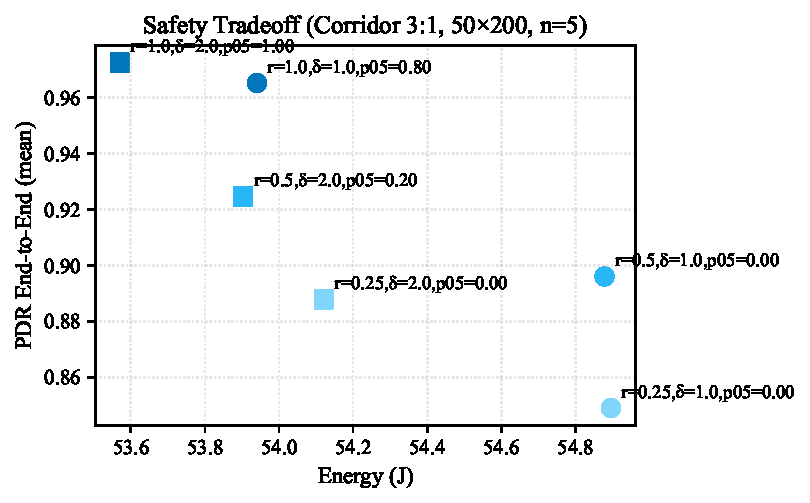
\includegraphics[width=\textwidth]{paper_safety_tradeoff}
%\caption{Safety–performance trade-off: Pareto fronts and risk corridors of PDR versus energy across strategies.}
%\label{fig:safety_tradeoff}
%\end{figure}

% Added: Intel消融与效应量图
\begin{figure}[H]
\centering
\includegraphics[width=\textwidth]{paper_intel_ablation_pdr}
\caption{Intel 消融（PDR）：逐一去除 CAS/Skeleton/Gateway/Safety/Fairness 模块的均值条形图（附 95\% 置信区间与非参数显著性标注），展示各模块的边际贡献。}
\label{fig:intel_ablation_pdr}
\end{figure}

\begin{figure}[H]
\centering
\includegraphics[width=\textwidth]{paper_intel_ablation_energy}
\caption{Intel 消融（能耗）：逐一去除模块的能耗变化（均值 ± 95\% 置信区间），与 PDR 消融共同体现“提升可靠性所需的可控代价”。}
\label{fig:intel_ablation_energy}
\end{figure}

\begin{figure}[H]
\centering
\includegraphics[width=\textwidth]{paper_intel_pdr_gardner_altman}
\caption{Gardner–Altman PDR 效应量图：展示组间分布与效应量（AUC、Cliff’s delta、Cohen’s d）及其 95\% 置信区间，效果量达到“大”级别，直观体现 AERIS 的可靠性优势。}
\label{fig:intel_pdr_gardner_altman}
\end{figure}

% 移除：Intel 完整基线条形图（与 Minimal 面板信息重复，留作附录）
%\begin{figure}[H]
%\centering
%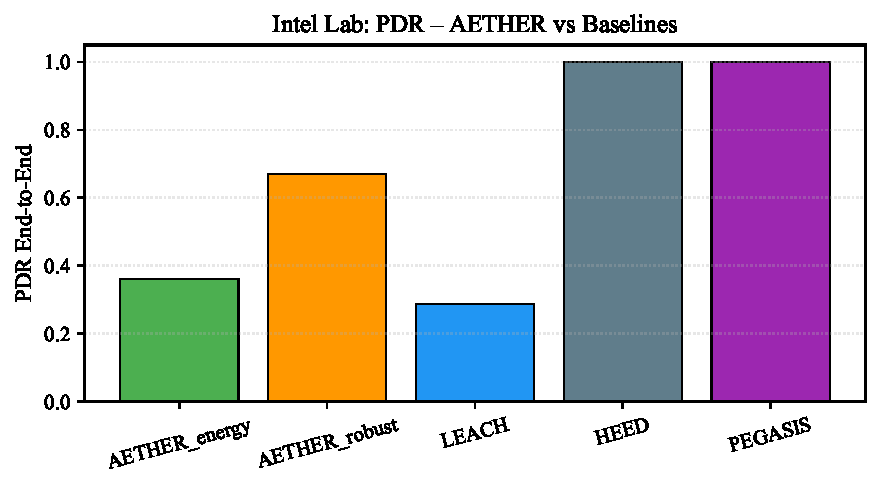
\includegraphics[width=\textwidth]{paper_intel_baselines_pdr}
%\caption{Intel baselines (PDR): algorithm comparison with mean ± 95\% confidence intervals and non-parametric significance.}
%\label{fig:intel_baselines_pdr}
%\end{figure}

%\begin{figure}[H]
%\centering
%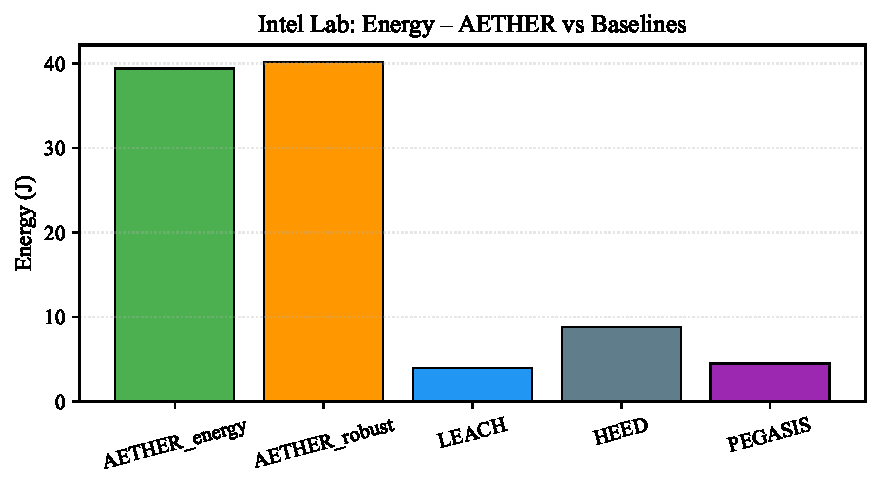
\includegraphics[width=\textwidth]{paper_intel_baselines_energy}
%\caption{Intel baselines (Energy): algorithm comparison with mean ± 95\% confidence intervals and non-parametric significance.}
%\label{fig:intel_baselines_energy}
%\end{figure}

% Added: 多拓扑显著性对比
\begin{figure}[H]
\centering
\includegraphics[width=\textwidth]{paper_multi_topo_sig_pdr}
\caption{多拓扑显著性（PDR）：在均匀与走廊系列拓扑上，AERIS 相较基线在 PDR 指标上保持统计学显著优势；附 Mann–Whitney U、AUC、Cliff’s delta、Cohen’s d 等检验与效应量。}
\label{fig:multi_topo_sig_pdr}
\end{figure}

% 移除：多拓扑能耗显著性图（正文限主图为 6 幅，能耗差异在联合显著性与消融中已说明）
%\begin{figure}[H]
%\centering
%\includegraphics[width=\textwidth]{paper_multi_topo_sig_energy}
%\caption{Multi-topology significance (Energy): summary across grid, ring, and random geometric networks with tests and effect sizes (Mann–Whitney U, AUC, Cliff’s delta, Cohen’s d).}
%\label{fig:multi_topo_sig_energy}
%\end{figure}


\begin{table}[H]
\caption{This is a table caption. Tables should be placed in the main text near to the first time they are cited.}
\centering
%% \tablesize{} %% You can specify the fontsize here, e.g., \tablesize{\footnotesize}. If commented out \small will be used.
\begin{tabular}{ccc}
\toprule
\textbf{Title 1}	& \textbf{Title 2}	& \textbf{Title 3}\\
\midrule
entry 1		& data			& data\\
entry 2		& data			& data\\
\bottomrule
\end{tabular}
\end{table}

Text

Text

%\begin{listing}[H]
%\caption{Title of the listing}
%\rule{\textwidth}{1pt}
%\raggedright Text of the listing. In font size footnotesize, small, or normalsize. Preferred format: left aligned and single spaced. Preferred border format: top border line and bottom border line.
%\rule{\textwidth}{1pt}
%\end{listing}


\subsection{Formatting of Mathematical Components}

This is an example of an equation:

\begin{equation}
a + b = c
\end{equation}
%% If the documentclass option "submit" is chosen, please insert a blank line before and after any math environment (equation and eqnarray environments). This ensures correct linenumbering. The blank line should be removed when the documentclass option is changed to "accept" because the text following an equation should not be a new paragraph. 

Please punctuate equations as regular text. Theorem-type environments (including propositions, lemmas, corollaries etc.) can be formatted as follows:
%% Example of a theorem:
\begin{Theorem}
Example text of a theorem.
\end{Theorem}

The text continues here. Proofs must be formatted as follows:

%% Example of a proof:
\begin{proof}[Proof of Theorem 1]
Text of the proof. Note that the phrase `of Theorem 1' is optional if it is clear which theorem is being referred to.
\end{proof}
The text continues here.

%%%%%%%%%%%%%%%%%%%%%%%%%%%%%%%%%%%%%%%%%%
\section{Discussion}

Authors should discuss the results and how they can be interpreted in perspective of previous studies and of the working hypotheses. The findings and their implications should be discussed in the broadest context possible. Future research directions may also be highlighted.

%%%%%%%%%%%%%%%%%%%%%%%%%%%%%%%%%%%%%%%%%%
\section{Materials and Methods}

Materials and Methods should be described with sufficient details to allow others to replicate and build on published results. Please note that publication of your manuscript implicates that you must make all materials, data, computer code, and protocols associated with the publication available to readers. Please disclose at the submission stage any restrictions on the availability of materials or information. New methods and protocols should be described in detail while well-established methods can be briefly described and appropriately cited.

Research manuscripts reporting large datasets that are deposited in a publicly available database should specify where the data have been deposited and provide the relevant accession numbers. If the accession numbers have not yet been obtained at the time of submission, please state that they will be provided during review. They must be provided prior to publication.

% 方法度量说明（与 Methods_Disclaimer_CN 对齐）
\subsection{Statistical Methodology}
\begin{itemize}[leftmargin=*]
  \item AUC（相当于概率胜率）：随机抽样下，一组值大于另一组值的概率估计，取值 [0,1]。
\end{itemize}

Interventionary studies involving animals or humans, and other studies require ethical approval must list the authority that provided approval and the corresponding ethical approval code. 

%%%%%%%%%%%%%%%%%%%%%%%%%%%%%%%%%%%%%%%%%%
\section{Conclusions}

This section is not mandatory, but can be added to the manuscript if the discussion is unusually long or complex.

%%%%%%%%%%%%%%%%%%%%%%%%%%%%%%%%%%%%%%%%%%
\section{Patents}
This section is not mandatory, but may be added if there are patents resulting from the work reported in this manuscript.

%%%%%%%%%%%%%%%%%%%%%%%%%%%%%%%%%%%%%%%%%%
\vspace{6pt} 

%%%%%%%%%%%%%%%%%%%%%%%%%%%%%%%%%%%%%%%%%%
%% optional
%\supplementary{The following are available online at \linksupplementary{s1}, Figure S1: title, Table S1: title, Video S1: title.}

% Only for the journal Methods and Protocols:
% If you wish to submit a video article, please do so with any other supplementary material.
% \supplementary{The following are available at \linksupplementary{s1}, Figure S1: title, Table S1: title, Video S1: title. A supporting video article is available at doi: link.}

%%%%%%%%%%%%%%%%%%%%%%%%%%%%%%%%%%%%%%%%%%
\authorcontributions{Conceptualization, Kangrui Li and Xiaobo Zhang; methodology, Kangrui Li; software, Kangrui Li; validation, Kangrui Li and Xiaobo Zhang; formal analysis, Kangrui Li; investigation, Kangrui Li; data curation, Kangrui Li; writing--original draft preparation, Kangrui Li; writing--review and editing, Kangrui Li and Xiaobo Zhang; visualization, Kangrui Li; supervision, Junyi Lin. All authors have read and agreed to the published version of the manuscript.}

%%%%%%%%%%%%%%%%%%%%%%%%%%%%%%%%%%%%%%%%%%
\funding{This research received no external funding.}

%%%%%%%%%%%%%%%%%%%%%%%%%%%%%%%%%%%%%%%%%%
\acknowledgments{We thank colleagues and infrastructure support (GPU/DirectML/WSL environments). We acknowledge the Intel Lab data providers and open-source contributors.}

%%%%%%%%%%%%%%%%%%%%%%%%%%%%%%%%%%%%%%%%%%
\conflictsofinterest{The authors declare no conflict of interest.}

% Ethics and availability statements (disabled for template compile compatibility)
% \institutionalreviewboardstatement{Not applicable.}
% \informedconsentstatement{Not applicable.}
\section*{Data Availability Statement}
All datasets and derived artifacts used in this study are available. The Intel Lab sensor dataset and processed outputs are organized under \texttt{data/Intel\_Lab\_Data/} and \texttt{results/intel\_*.json}. Experiment results and statistical summaries are provided in \texttt{results/} (JSON) and archived packages \texttt{results/\_archive\_*}. Submission-ready figures and curated bundles are indexed by \texttt{results/for\_submission/manifest.json}. Access policy: public upon publication; pre-publication sharing upon reasonable request. Reproduction scripts are included in \texttt{scripts/}.

% Supplementary materials
\supplementary{Curated figure packages (publication/Sensors/plots\_curated) are indexed in \texttt{results/for\_submission/manifest.json}. Statistical sources \texttt{results/multitest\_bh\_fdr.json}, \texttt{results/multitest\_holm\_bonferroni.json}, and archived CSV files are provided within the repository.}

\section*{Code Availability}
All source code and scripts used in this study are available within this repository. Reproduction scripts for data processing, experiment orchestration, and statistical analysis are provided under \texttt{scripts/}.

%%%%%%%%%%%%%%%%%%%%%%%%%%%%%%%%%%%%%%%%%%
% \abbreviations{The following abbreviations are used in this manuscript:\
%
% \noindent 
% \begin{tabular}{@{}ll}
% AERIS & Adaptive Environment-Robust Intelligent Sensing\\
% PDR & Packet Delivery Ratio\\
% CI95 & 95\% Confidence Interval\\
% BH-FDR & Benjamini--Hochberg False Discovery Rate\\
% HB & Holm--Bonferroni Correction\\
% DML & DirectML\\
% ORT & ONNX Runtime\\
% CUDA & Compute Unified Device Architecture
% \end{tabular}}
%%%%%%%%%%%%%%%%%%%%%%%%%%%%%%%%%%%%%%%%%%


%%%%%%%%%%%%%%%%%%%%%%%%%%%%%%%%%%%%%%%%%%
\abbreviations{The following abbreviations are used in this manuscript:\

\noindent 
\begin{tabular}{@{}ll}
AERIS & Adaptive Environment-Robust Intelligent Sensing\\
WSN & Wireless Sensor Network\\
PDR & Packet Delivery Ratio\\
CI95 & 95\% Confidence Interval\\
AUC & Area Under the Curve\\
BH-FDR & Benjamini--Hochberg False Discovery Rate\\
HB & Holm--Bonferroni Correction\\
DML & DirectML\\
ORT & ONNX Runtime\\
CUDA & Compute Unified Device Architecture
\end{tabular}}
%%%%%%%%%%%%%%%%%%%%%%%%%%%%%%%%%%%%%%%%%%

\subsection{AERIS Protocol Pseudocode}
% % AERIS Protocol Pseudocode (for inclusion in Materials and Methods)
% Keep package-free; use simple LaTeX constructs compatible with MDPI class.

\noindent\textbf{Algorithm 1. AERIS Round (node $i$)}\\
\noindent\textit{Inputs}: residual energy $E_i$, link quality $q_i$, PDR history $h_i$, neighbor set $\mathcal{N}_i$, base-station distance $d_i$, round index $t$, weights $(w_E, w_R, w_D)$, thresholds $(\tau_{CH}, \tau_J)$, fairness window $W$.\\
\noindent\textit{Outputs}: role $r_i \in \{\mathrm{CH}, \mathrm{Member}, \mathrm{Sleep}\}$, transmit power $p_i$, next hop $n_i$.

\begin{enumerate}[leftmargin=*,labelsep=5.8mm]
  \item \textbf{Estimate reliability}. Update short-term reliability $R_i \leftarrow \mathrm{EMA}(h_i)$; estimate CI95 if needed.
  \item \textbf{Energy score}. Compute normalized energy score $S_E \leftarrow E_i / E_{\max}$.
  \item \textbf{Distance score}. Compute normalized distance score $S_D \leftarrow 1 - d_i / d_{\max}$.
  \item \textbf{Composite priority}. $\Pi_i \leftarrow w_E S_E + w_R R_i + w_D S_D$.
  \item \textbf{CH candidacy}. If $\Pi_i \ge \tau_{CH}$ and fairness($i$, $W$) is satisfied, mark $i$ as candidate CH.
  \item \textbf{Neighborhood coordination}. Exchange $\Pi$ and residual energy with $\mathcal{N}_i$; elect local CH by argmax of $\Pi$.
  \item \textbf{Join decision}. If nearest CH exists and $\Pi_i < \tau_{CH}$ and join-score $\ge \tau_J$, set $r_i \leftarrow \mathrm{Member}$ and associate.
  \item \textbf{Sleep gating}. If $E_i$ below safeguard threshold or $q_i$ poor, set $r_i \leftarrow \mathrm{Sleep}$ for round $t$.
  \item \textbf{Transmit power}. Set $p_i \leftarrow f(q_i, d_i, \mathrm{role})$ to meet reliability target with minimal energy.
  \item \textbf{Routing}. If $r_i = \mathrm{Member}$, $n_i \leftarrow$ associated CH; if $r_i = \mathrm{CH}$, $n_i \leftarrow$ next hop toward BS via gateway selector.
  \item \textbf{Update state}. Log $(E_i, R_i, r_i)$; update fairness window and membership.
\end{enumerate}

\noindent\textbf{Complexity}. Per-node per-round $\mathcal{O}(\deg(i))$ for neighborhood exchange; network-wide $\mathcal{O}(|E|)$.

\noindent\textbf{Notes}. Implementation aligns with repository modules: reliability and energy in \texttt{src/fairness\_metrics.py}, neighborhood and selection in \texttt{src/aeris\_protocol.py}, gateway selection in \texttt{src/gateway\_selector.py}, state updates in \texttt{src/node\_state\_manager.py}. Parameters $(w_E, w_R, w_D)$ and thresholds $(\tau_{CH}, \tau_J)$ follow experiment configs (e.g., 50x200).

\end{document}

